%*****************************************
\chapter{Sampling}\label{07:sampling}
%*****************************************
%TODO Status: Pre-draft

\begin{wrapfigure}{O}{0.4\textwidth}
	\label{07:fig01} 
	\centering
	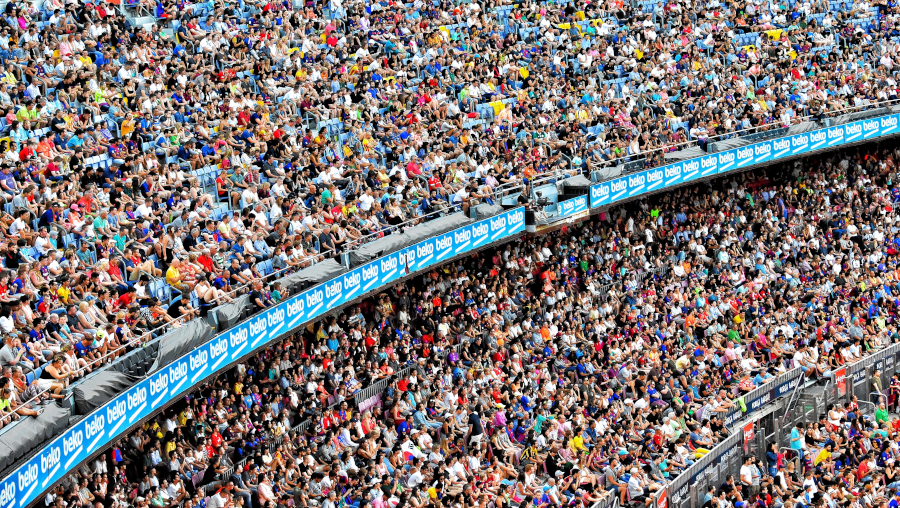
\includegraphics[width=0.4\textwidth]{gfx/07-01} 
\end{wrapfigure}
Imagine that a research team undertakes a project to determine the number of t-shirts to order for an upcoming promotion in a large stadium. The question that the stadium owner needs answered is how many small/medium/large t-shirts should be ordered. To figure that out, the researchers decide to conduct a survey of the fans a few weeks before the promotion and ask them what size t-shirt they would prefer. So, how many fans should they survey? They could ask every fan in the stadium if they hired enough poll-takers, but that would be expensive and wasteful. Perhaps it is enough to ask $ 10\% $ of the crowd -- maybe just $ 1\% $. Once the researchers figure out how many people to survey, then they need to figure out how to select those people. Do they select everyone in a specific section? Do they ask the first $ 100 $ people who come through a specific gate? These are questions that concern sampling and whatever decisions the researchers make concerning the stadium crowd may profoundly change the data that are collected, and not necessarily for the best. This chapter concerns sampling and offers information about how to determine a sample size and what techniques can be used to reduce bias in the sample.
\blfootnote{Photo by Ekansh Saxena on Unsplash}

\section{Introduction}

Business and marketing research generally concerns inferring patterns of behaviors within specific populations where a \gls{population} is a cluster of people, events, things, or other phenomena of interest. Unfortunately, populations may be rather large and vaguely defined, such as ``the American people,'' or ``grocery stores in the United States.'' Even those populations that are not so vague can also be too large to study directly, like all shoppers over the age of $ 18 $ within a specific region. Normally, it is not feasible to study an entire population because of cost constraints so a representative sample is selected from the population for observation and analysis. 

A \gls{sample} is a small subset of the population from which data are gathered in order to make statistical inferences about the entire population. Sampling strategies are designed to allow researchers to make claims about populations that are much larger than they actually sample with a fair amount of confidence. It is extremely important for researchers to choose a sample that is truly representative of the population so the inferences derived can be generalized back to the entire population. Improper and biased sampling is the primary reason for the often divergent and erroneous inferences reported in opinion polls conducted by different groups prior to every United States Presidential election.

The sampling process involves several stages. 

\begin{enumerate}
	\item Defining the target population. A population can be defined as all people or items (unit of analysis) with the characteristic of interest. The unit of analysis may be a person, group, organization, country, object, or any other entity about which scientific inferences can be drawn. Sometimes the population is obvious. For example, if a manufacturer wants to determine whether finished goods manufactured on a particular production line meet certain quality specifications then the population consists of the entire set of finished goods manufactured on that line. At other times the target population may be a little harder to understand. If the research project is to identify the primary motivators of shopping behavior among high school students then the target population may be high school students, store managers who are selling products to those students, or even the product manufacturers who design the packaging. 

	\item Determine the \gls{sampleframe}. This is an accessible section of the target population (often a list with contact information) from which a sample can be drawn. If the target population is ``professional employees'' then the sampling frame would likely be the professional employees at a local company since it would not be possible to access all professional employees around the world. If the target population is ``business organizations'' then the Fortune $ 500 $ list may be an acceptable sampling frame.

	Note that sampling frames may not be representative of the population at large so inferences derived by that sample may not be generalizable to the population. For instance, if the target population is the employees of small businesses and the sampling frame is employees at automotive tire companies in the American Midwest then findings from that group may not be generalizable to the American workforce at large, let alone the global workplace. Similarly, the Fortune $ 500 $ list includes the $ 500 $ largest American enterprises, which is not representative of American firms in general, most of which are medium and small-sized firms. Also note that the population from which a sample is drawn may not necessarily be the same as the population about which the research is targeted. For example, if a researcher wants to the success rate of a new ``quit smoking'' program, then the target population is the universe of smokers who had access to this program, which may be an unknown population. Hence, the researcher may sample patients arriving at a local medical facility for smoking cessation treatment, some of whom may not have had exposure to this particular ``quit smoking'' program, in which case, the sampling frame does not correspond to the population of interest.

	\item Select a sample. Once the sampling frame is defined the actual sample must be drawn using a well-defined technique. Sampling techniques can be grouped into two categories: \gls{probabilitysampling} (or random) sampling and \gls{nonprobibilitysampling} sampling. Probability sampling is important if the results are to be generalized but there may be unique circumstances where non-probability sampling can also be justified.

\end{enumerate}

As an example of this process, consider Figure \ref{07:fig11}\footnote{Photo of the population by not brittany shh pls on Unsplash. Photo of the list by Sophia Baboolal on Unsplash. Photo of the two men by rawpixel on Unsplash}. Imagine that a researcher intends to conduct some sort of project where the intent is to draw some conclusions about professional workers around the world. That population would be much too large to survey directly, so a sampling frame would be created of, perhaps, the professional workers at two or three local companies. From that frame, specific workers would be selected for observation.

\begin{figure}[H]
	\centering
	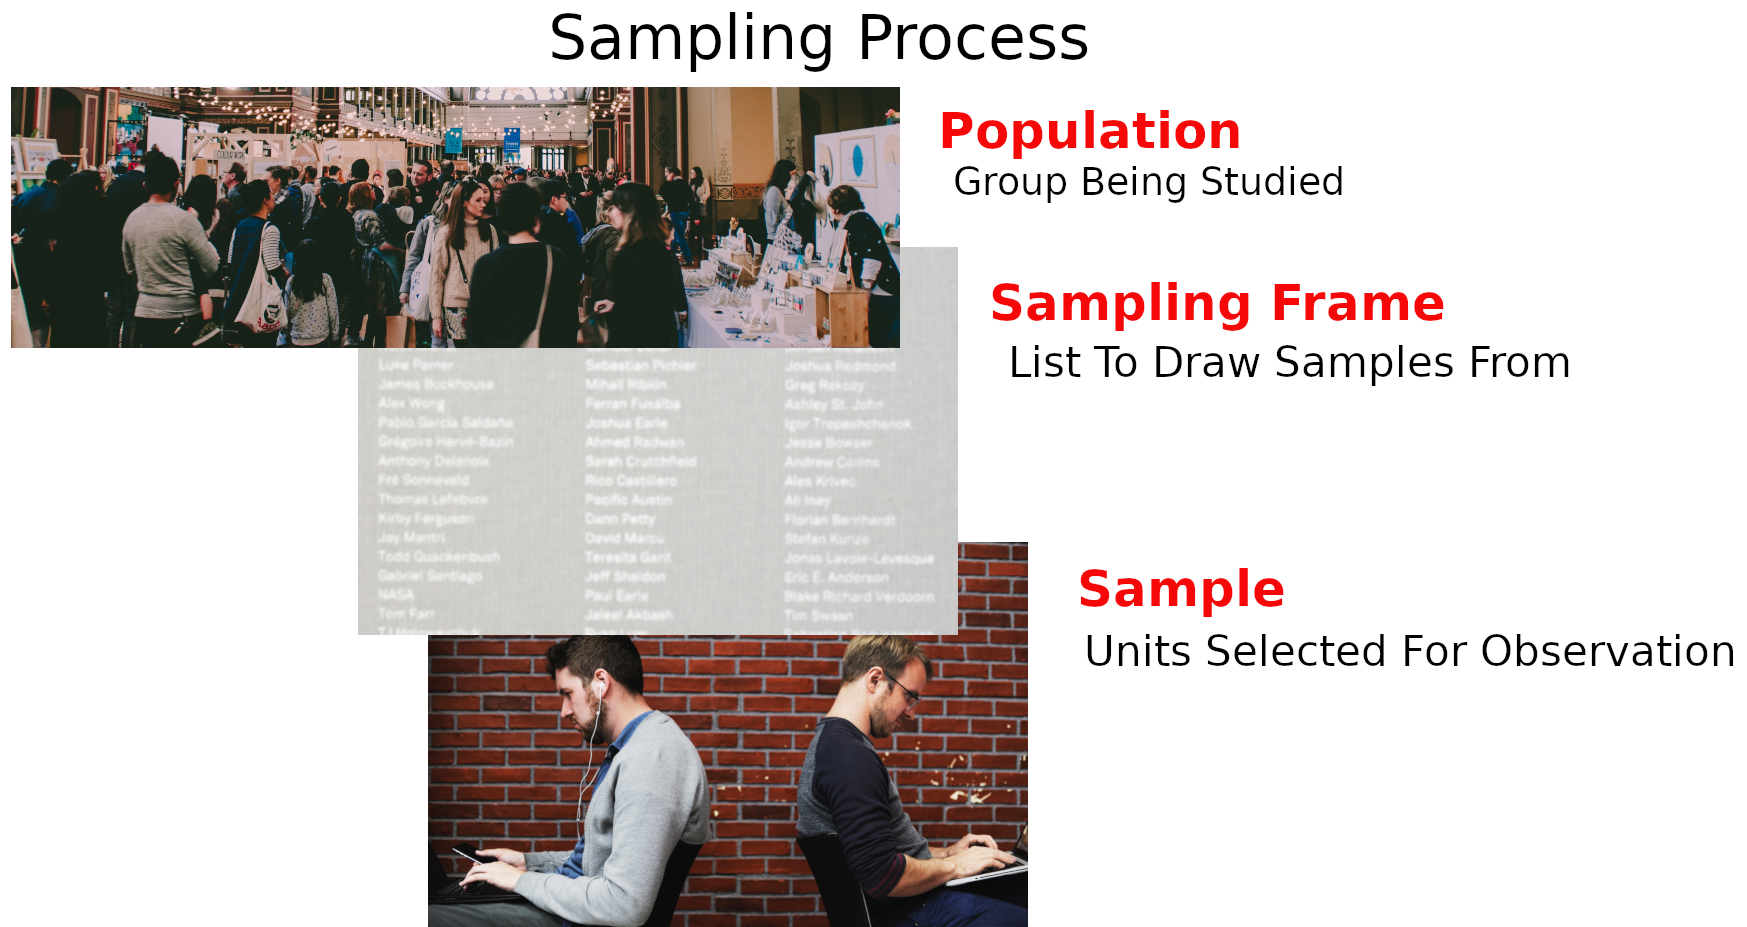
\includegraphics[width=\maxwidth{.95\linewidth}]{gfx/07-11}
	\caption{Sampling Process Visualized}
	\label{07:fig11}
\end{figure}

Both qualitative and quantitative researchers use sampling techniques but because the goals of qualitative and quantitative research differ the sampling procedures employed are also different.

\section{Sampling in Quantitative Research}

Quantitative researchers are often interested in being able to make generalizations about populations that are larger than their study samples and rely on \gls{probabilitysampling}. Probability sampling is a technique in which every unit in the population has a chance (non-zero probability) of being selected to be sampled and this chance can be accurately determined. It is important that every element in the sample frame has a known chance to be sampled because that makes the sample representative of the entire population. If, for example, a researcher is investigating something about the differences between men and women shoppers then it would be important that the sample contained both men and women in about the same proportions as in the entire population. This is a bit of an over-simplification but it points out the importance of a representative sample. Obtaining a representative sample is also important because a key goal of studies that rely on probability samples is generalizability. In fact, generalizability is perhaps the key feature that distinguishes probability samples from non-probability samples. Generalizability refers to the idea that the results will indicate something about the entire population.

One goal for a parametric sample is that it forms a normal distribution and has negligible skew and excess kurtosis \footnote{See Chapter \ref{06:data} for a definition of skew and excess kurtosis}. Statistics that are generated from the sample, such as the mean or standard deviation, are unbiased estimates of population parameters as long as the samples are selected properly. Therefore, statistical analysis of the sample can be reasonably applied to the entire population. All probability sampling has two attributes in common: 1) every unit in the population has a known non-zero probability of being sampled, and 2) the sampling procedure involves random selection. The different types of probability sampling techniques include the following.

\textbf{Simple Random Sampling} In this technique, all possible subsets of a population (more accurately, of the sampling frame) have an equal probability of being selected, making the sample an unbiased estimate of the population. 

Simple random sampling involves randomly selecting respondents from a sampling frame, usually employing a table of random numbers\footnote{A table of random numbers can be generated at \url{http://stattrek.com/Tables/Random.aspx}.} or a computerized random number generator. For instance, to randomly select $ 200 $ firms to survey from a list of $ 1000 $ firms the list could be entered into a spreadsheet program like Excel then the ``random'' function could be used to generate a random number for each of the $ 1000 $ firms. Next, the list is sorted by the random number and the first $ 200 $ firms on that sorted list would be selected. This is the simplest of all probability sampling techniques and that simplicity is also its greatest strength. Because the sampling frame is not subdivided or partitioned, the sample is unbiased and the inferences are the most generalizable when compared to other probability sampling techniques.

Figure \ref{07:fig02} illustrates simple random sampling. A few individuals in the entire population are selected (circled) at random for the study.

\begin{figure}[H]
	\centering
	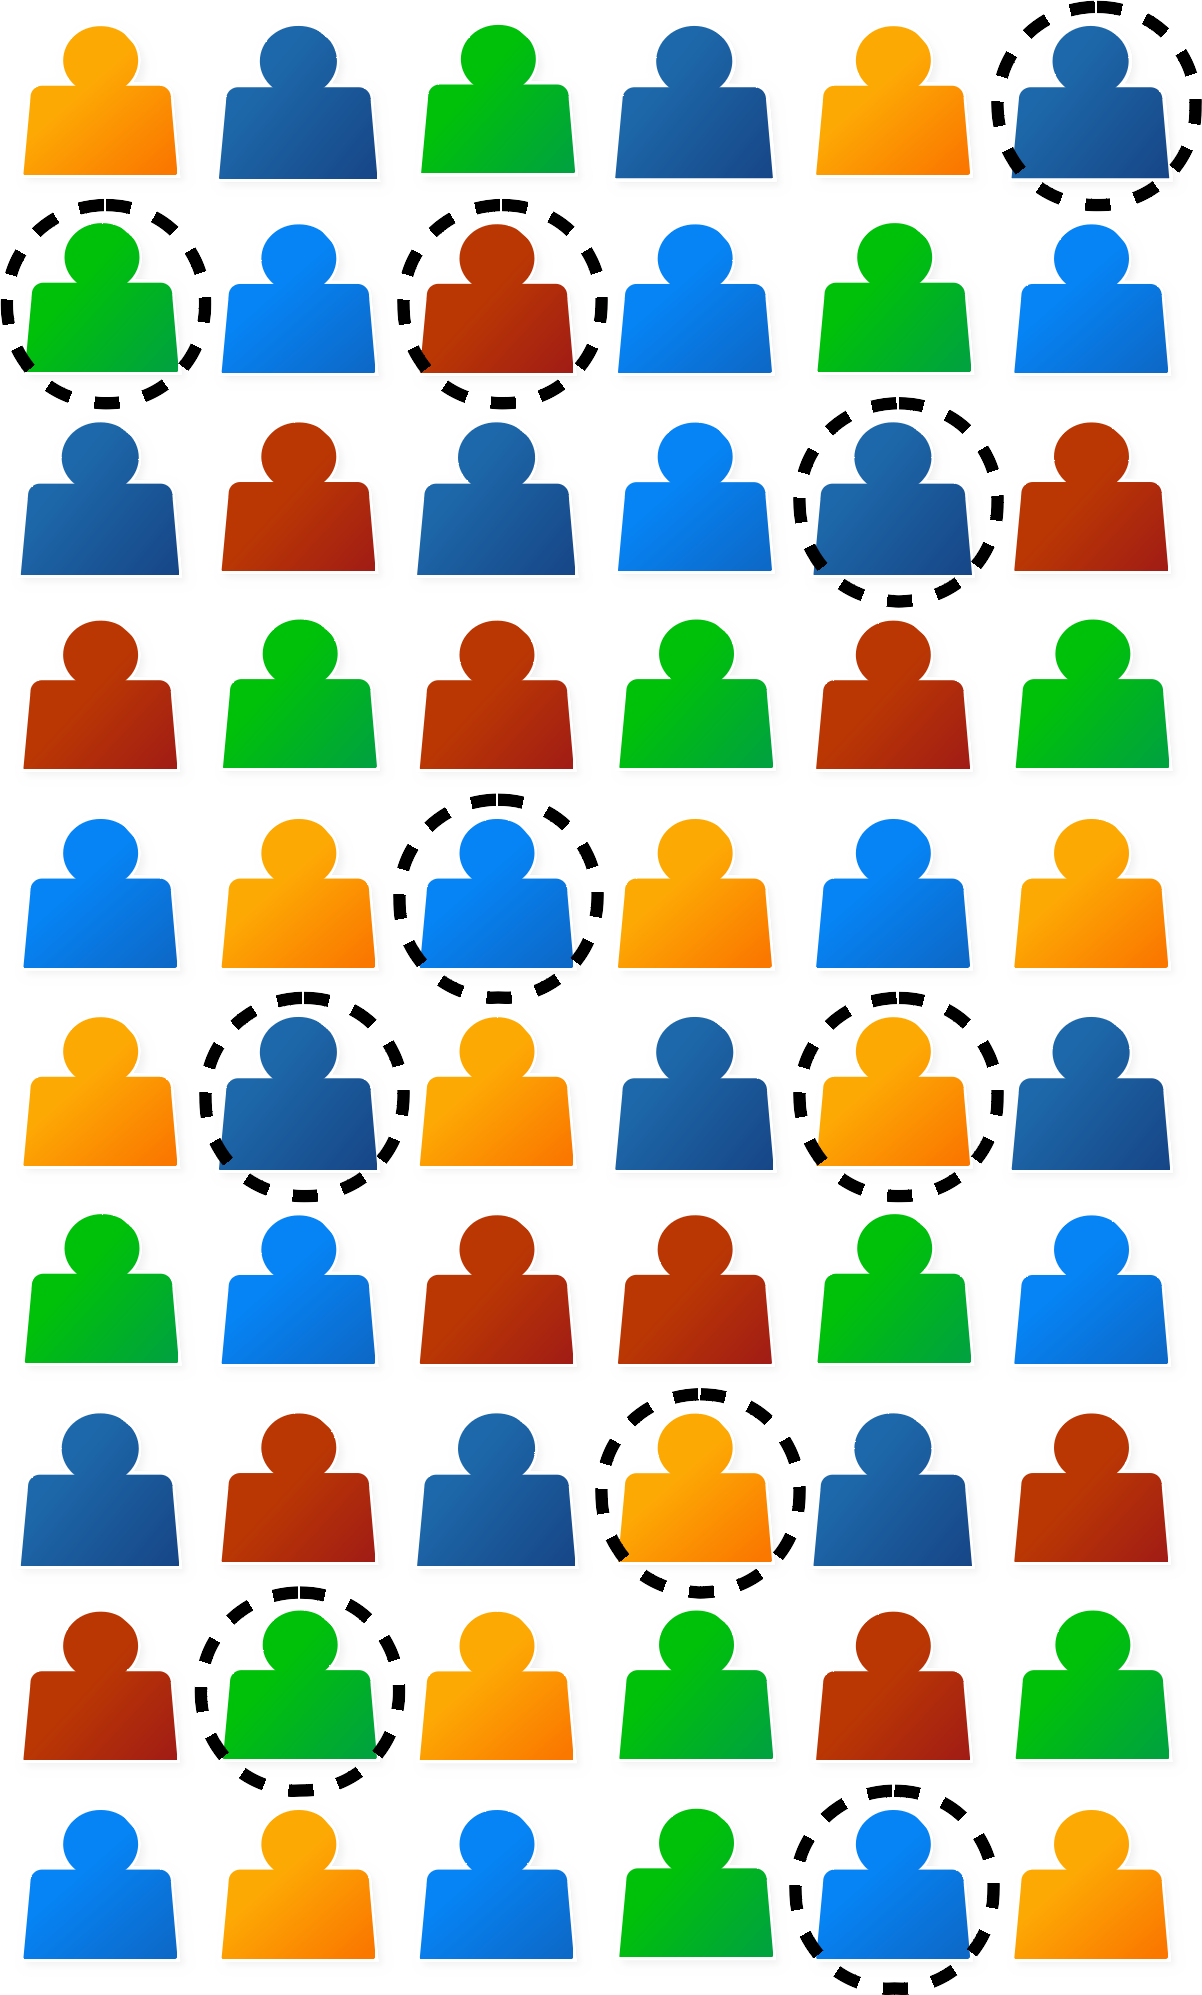
\includegraphics[width=\maxwidth{.35\linewidth}]{gfx/07-02}
	\caption{Simple Random Sampling}
	\label{07:fig02}
\end{figure}

\textbf{Systematic Sampling} In this technique, the sampling frame is ordered according to some criteria and then elements are selected at regular intervals through that ordered list. Systematic sampling involves a random start and then proceeds with the selection of every \textit{kth} element from that point onwards. The value of \textit{k} is easily calculated by $ k = N/n $, where \textit{k} (the sampling ratio) is calculated by dividing the size of the sampling frame, \textit{N}, by the desired number of samples, \textit{n}. It is important that the starting point is not automatically the first item in the list, but is instead randomly chosen from within the first \textit{k} elements on the list. Using the previous example of selecting $ 200 $ firms from a list of $ 1000 $, \textit{k} is equal to $ 5 $ ($ k = 1000/200 $). The list of $ 1000 $ firms would be sorted in increasing (or decreasing) order by some size-related criterion, like employee count or annual revenues. Then, one of the first five (the value of \textit{k}) firms on the list would be randomly selected and every fifth firm after that. This process ensures that there is no over-representation of large or small firms in the sample but, rather, that firms of all sizes are generally uniformly represented. In other words, the sample is representative of the population, at least on the basis of the sorting criterion.
	
There is one clear instance in which systematic sampling should be avoided. If the sampling frame has a pattern then bias can be introduced with a systemic sampling strategy. This is sometimes referred to as the problem of \textit{periodicity}, which is the tendency for a pattern to occur at regular intervals. Imagine, for example, that a researcher wanted to observe how people use the outdoor spaces on a college campus. Perhaps the researcher selects ``random'' dates in the month of September to make observations but due to the way the weekdays cycle it is possible (perhaps even likely) that all observations will be on the same day of the week. When working with patterned data it is best to not use systematic sampling.

Figure \ref{07:fig03} illustrates systematic sampling. In this case, $ k = 5 $ so every fifth person is chosen. At random, person three was chosen to start the pattern and then every fifth person after that is chosen.

\begin{figure}[H]
	\centering
	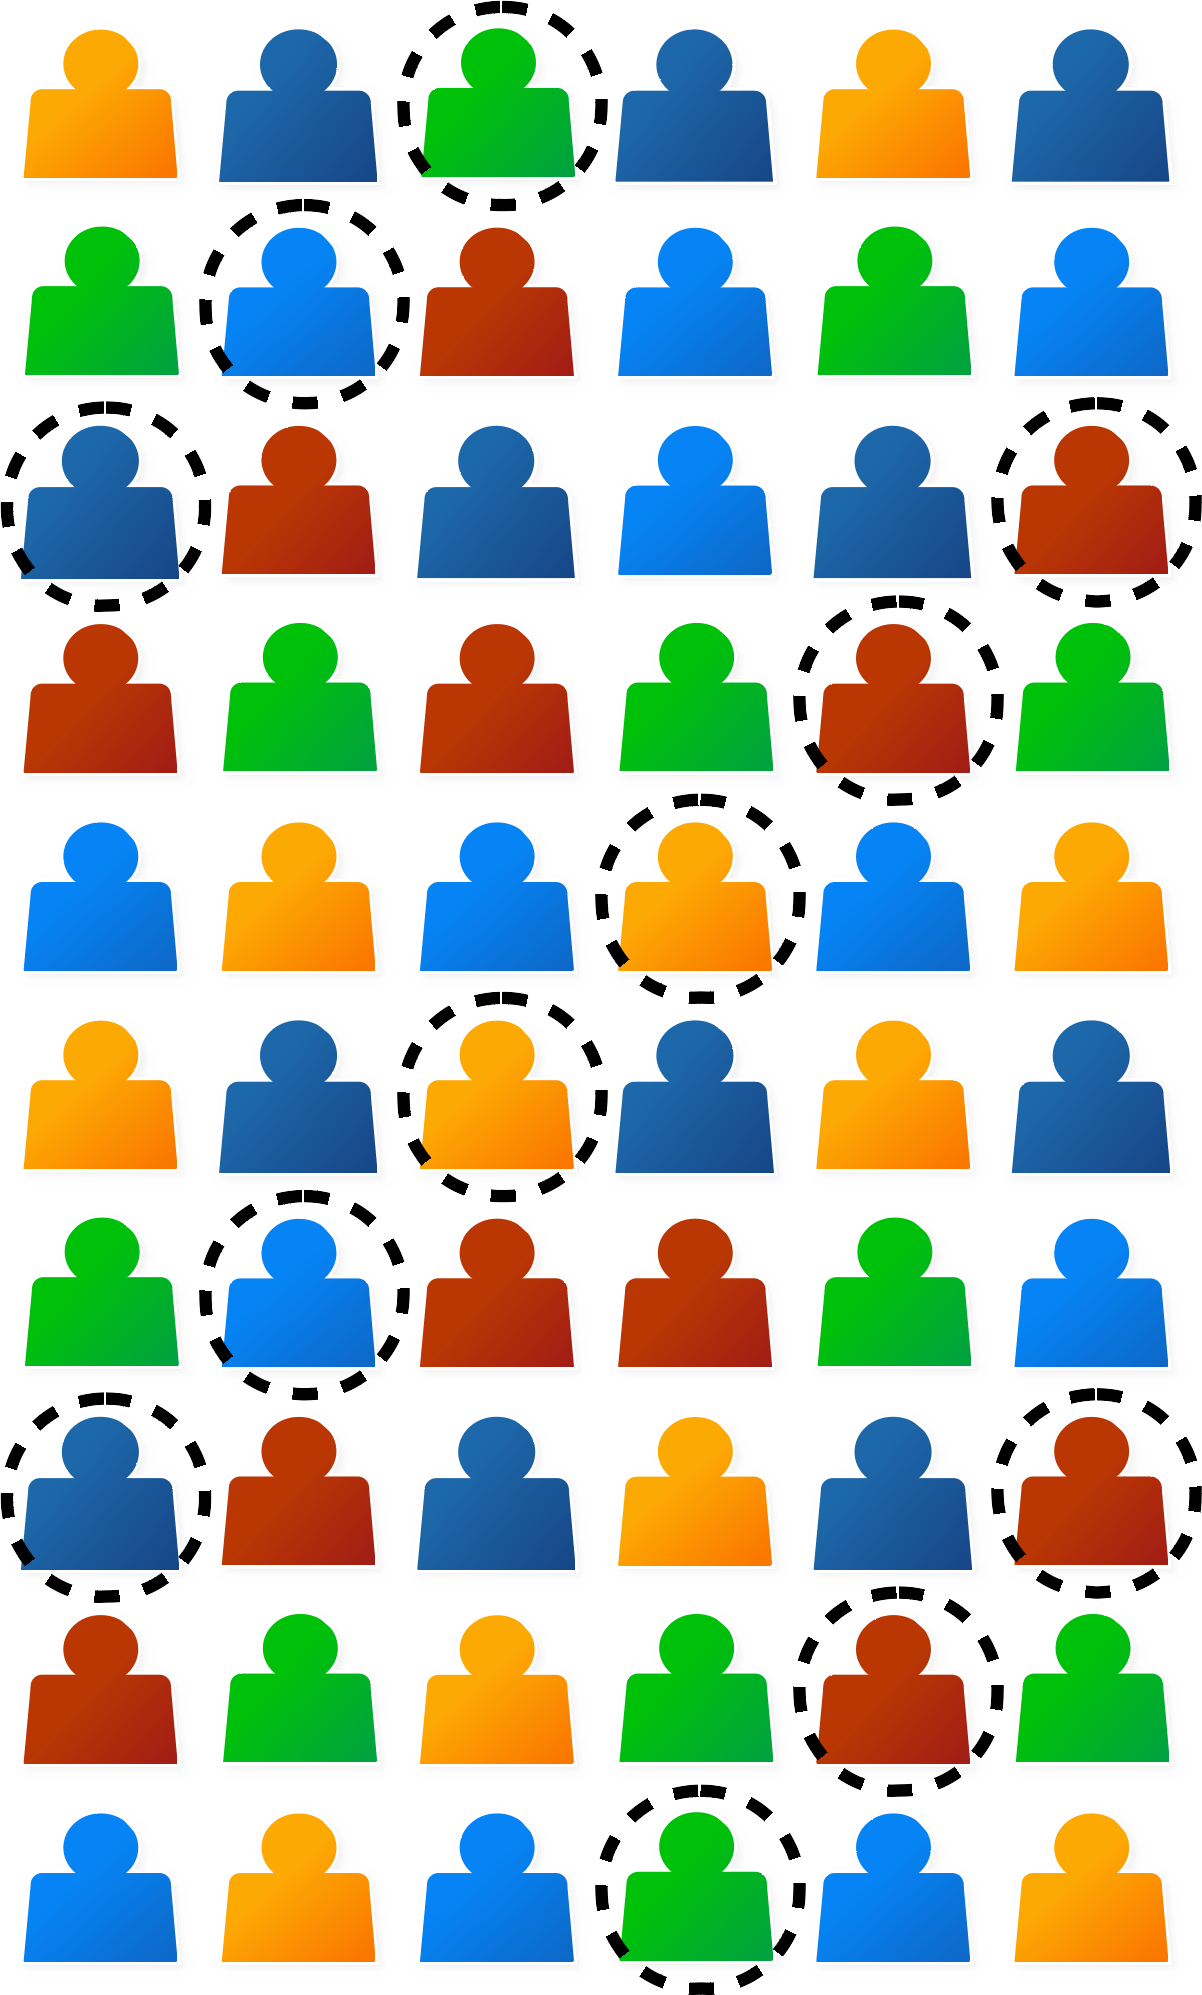
\includegraphics[width=\maxwidth{.35\linewidth}]{gfx/07-03}
	\caption{Systematic Sampling}
	\label{07:fig03}
\end{figure}

\textbf{Stratified Sampling} In stratified sampling, the sampling frame is divided into homogeneous and non-overlapping subgroups, called ``strata,'' and a simple random sample is drawn from each subgroup. Using the previous example of selecting $ 200 $ firms from a list of $ 1000 $, the firms could be categorized by size, perhaps ``large'' (more than $ 500 $ employees), ``medium'' ($ 50 - 500 $ employees), and ``small'' (fewer than $ 50 $ employees). Then, $ 67 $ firms would be randomly selected from each subgroup to create a sample of $ 200 $ firms. However, since there are many more small firms in a sampling frame than large firms, having an equal number of small, medium, and large firms will make the sample less representative of the population (in this case, biased in favor of large firms that are fewer in number in the target population). This is called non-proportional stratified sampling because the proportion of sample within each subgroup does not reflect the proportions in the sampling frame (or the population of interest), and the smaller subgroup (large-sized firms) is oversampled. 
	
An alternative technique is to select subgroup samples in proportion to their numbers in the population. For instance, if there are $ 100 $ ``large'' firms, $ 300 $ ``medium'' firms, and $ 600 $ ``small'' firms, then $ 20 $ should be selected from the ``large'' group, $ 60 $ from the ``medium'' group and $ 120 $ from the ``small'' group in order to maintain the correct proportion of firms. This technique is called \textit{proportional stratified sampling}. Note that the non-proportional approach is particularly effective in representing subgroups with fewer elements, such as large-sized firms in this example, but each subgroup's results must be weighted by its proportion in the population.

Figure \ref{07:fig04} illustrates stratified sampling. The population is divided into five subgroups and three elements were chosen from each subgroup. This would be an example of non-proportional stratified sampling since the same number are selected from each subgroup, though, in this case, each subgroup is the same size.

\begin{figure}[H]
	\centering
	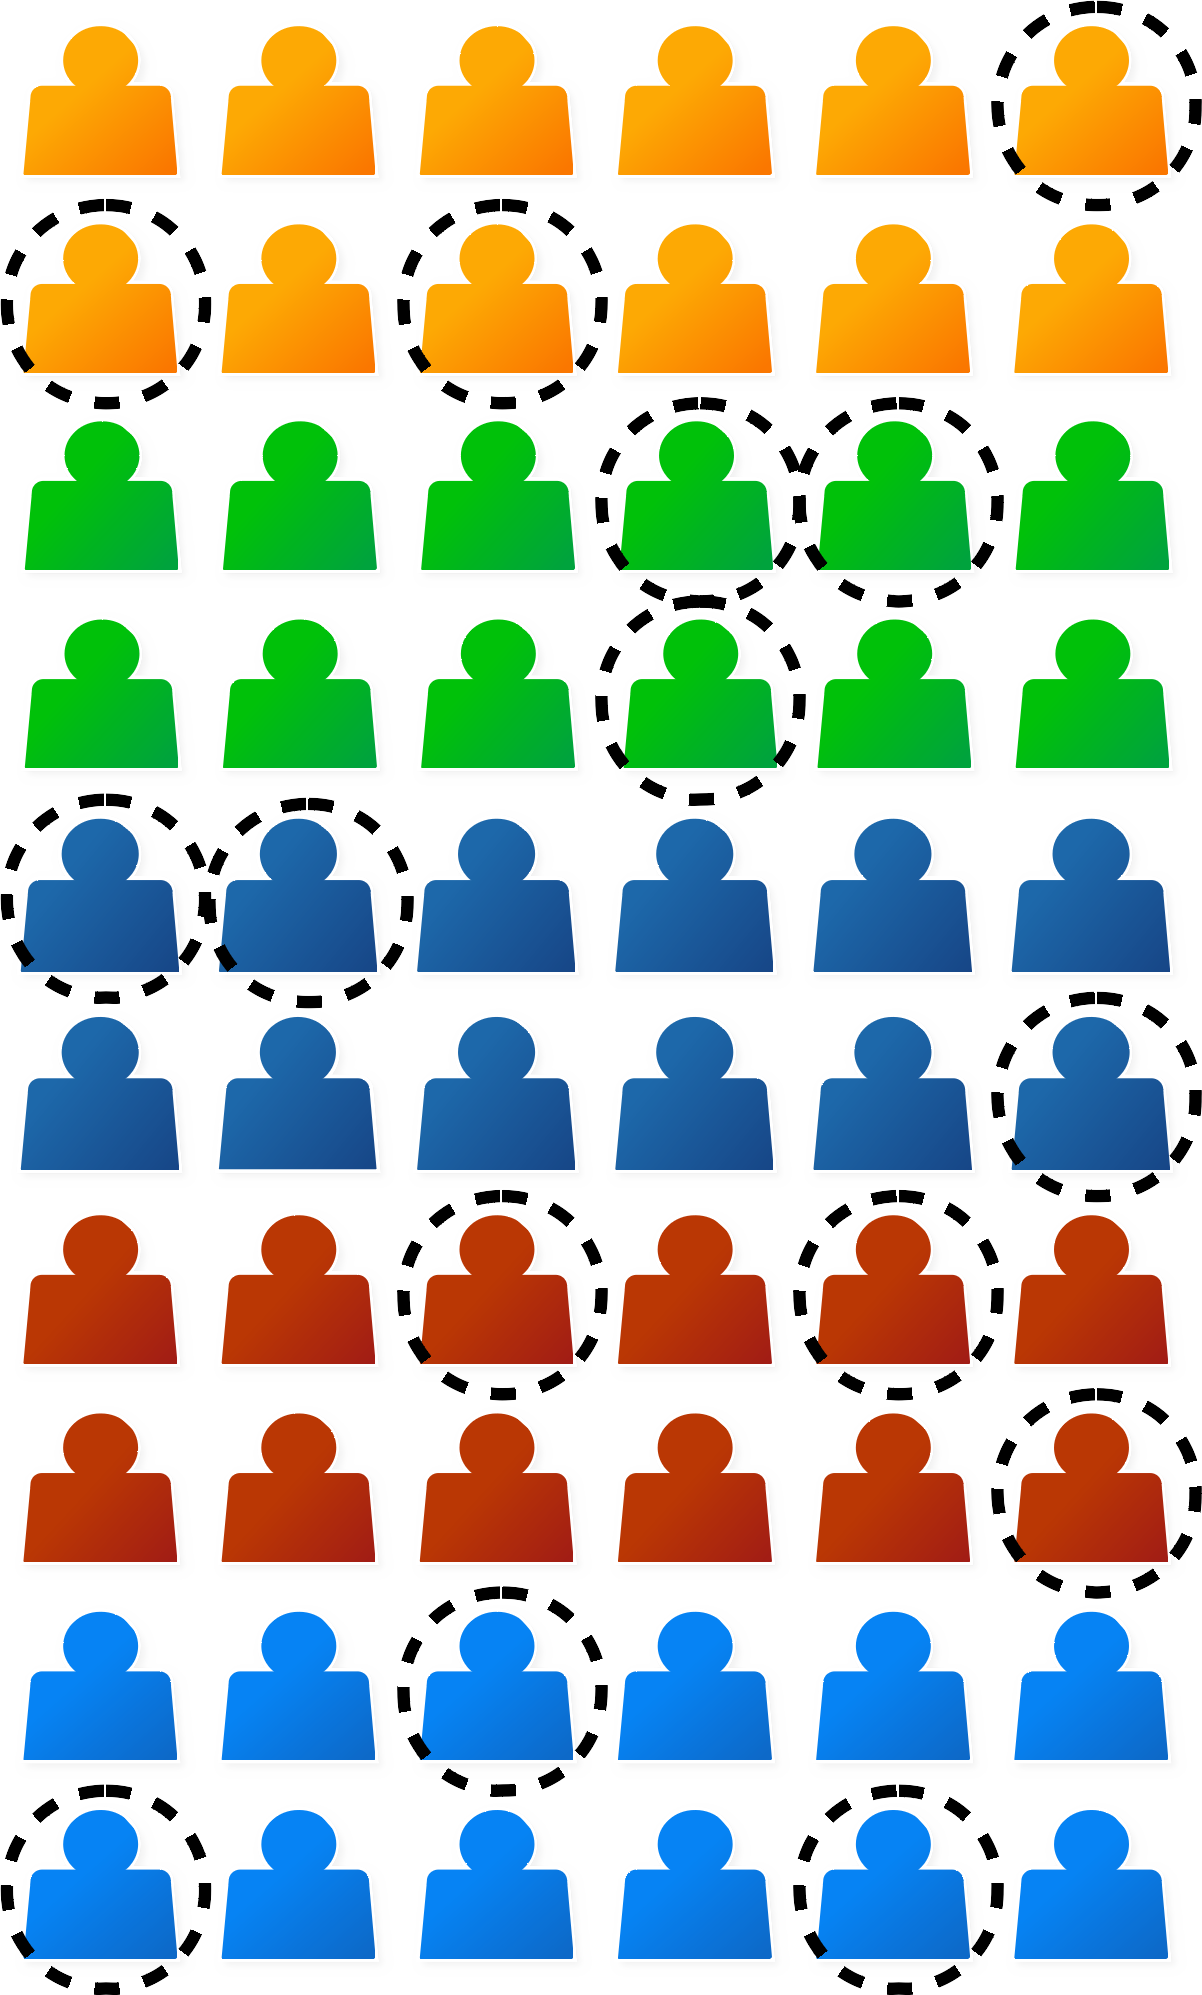
\includegraphics[width=\maxwidth{.35\linewidth}]{gfx/07-04}
	\caption{Stratified Sampling}
	\label{07:fig04}
\end{figure}

\textbf{Cluster Sampling} If the population is dispersed over a wide geographic region it may not be feasible to conduct a simple random sampling of the entire population. In such case, it may be reasonable to divide the population into ``clusters'' (typically along geographic boundaries), randomly select only a few clusters, and then measure all units within that cluster. For instance, to sample city governments in the state of New York, rather than travel all over the state to interview key city officials (as would be necessary with a simple random sample), the cities could be clustered by county and then all city officials in a randomly-selected group of counties would be interviewed. However, depending on between-cluster differences, the variability of sample results from a cluster sample will generally be higher than for a simple random sample so the results would be less generalizable to the population.

Figure \ref{07:fig05} illustrates cluster sampling. In this case, the population was divided into five clusters and then clusters three and four were randomly selected for the research project.

\begin{figure}[H]
	\centering
	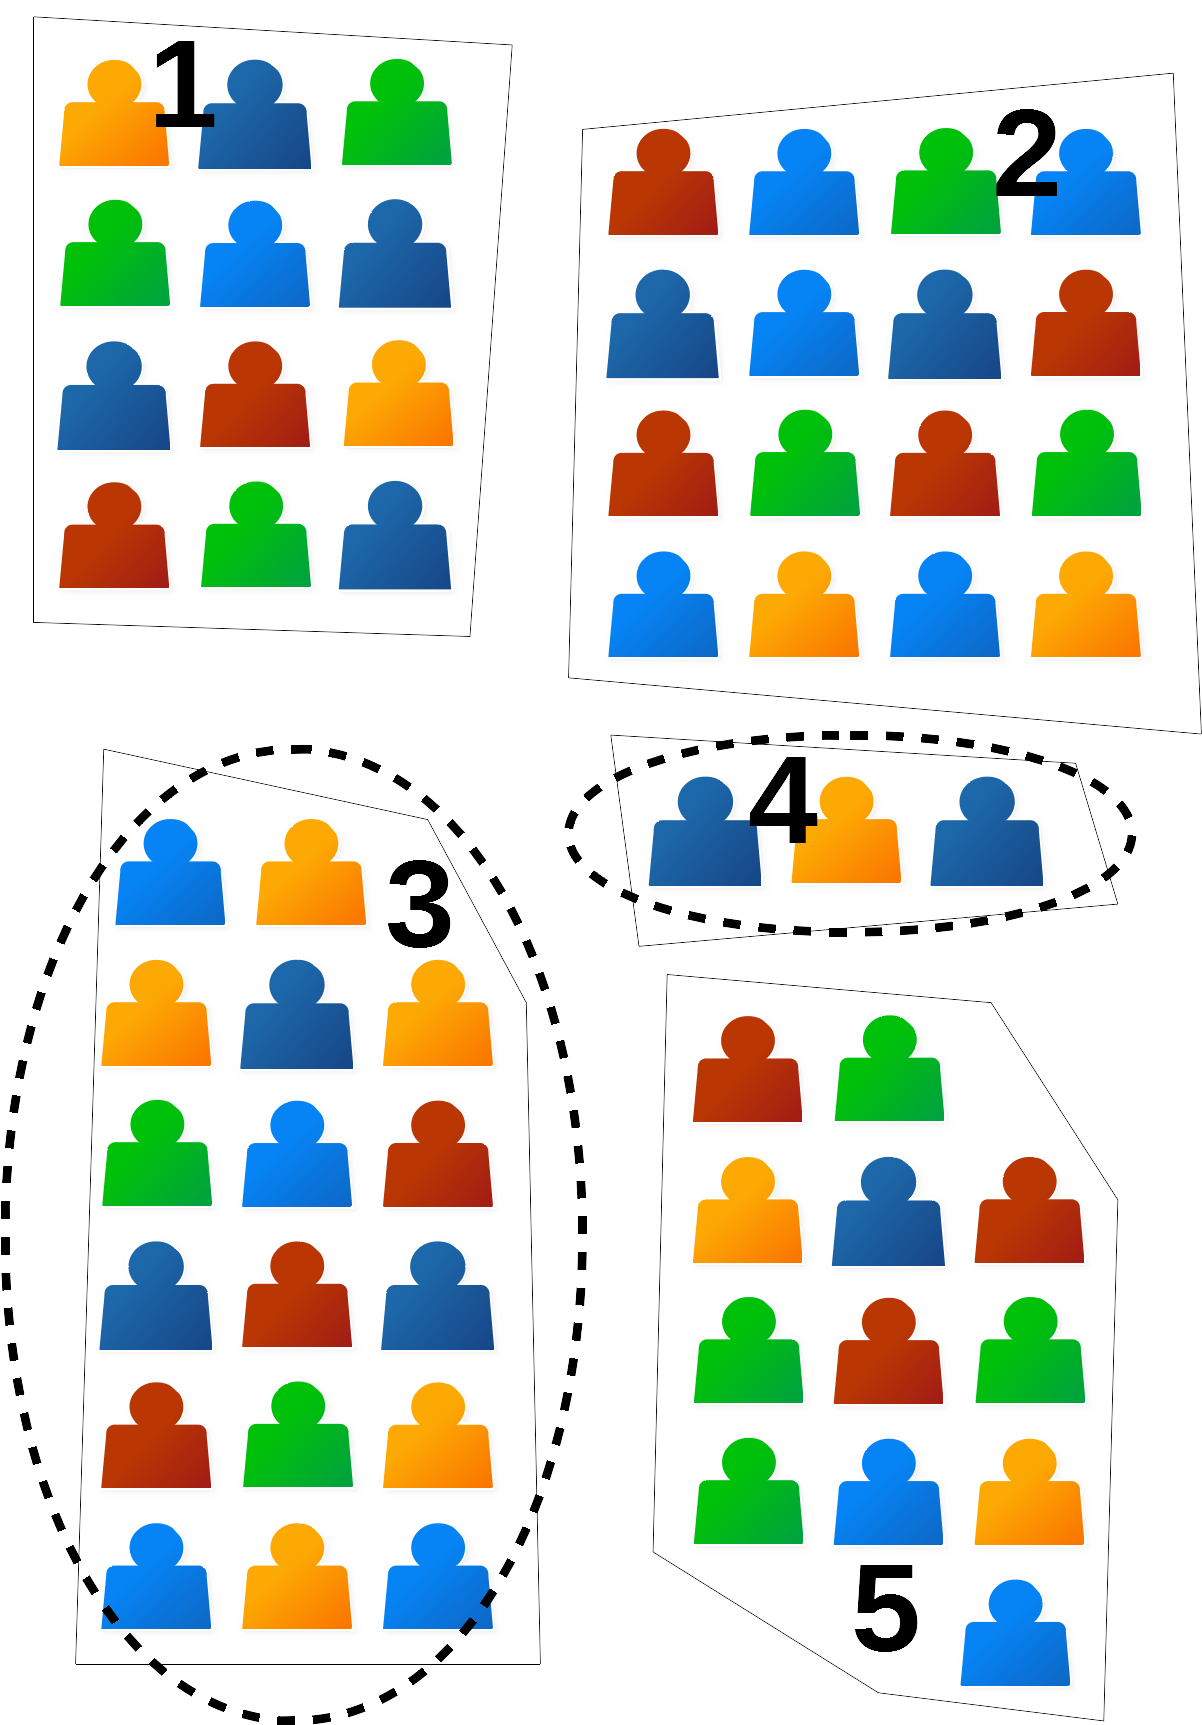
\includegraphics[width=\maxwidth{.35\linewidth}]{gfx/07-05}
	\caption{Cluster Sampling}
	\label{07:fig05}
\end{figure}

\textbf{Matched-pair Sampling} Sometimes, researchers may want to compare two subgroups within one population based on a specific criterion; for example, why are some firms consistently more profitable than others? To conduct such a study, the sampling frame of firms would be categorized into ``high profitable'' and ``low profitable'' firms based on gross margins, earnings per share, or some other measure of profitability. Then, a simple random sample of firms in one subgroup is selected. Each of those firms would be matched with one in the other subgroup based on its size, industry segment, or other criteria. Now, each of the firms can be studied in greater detail to look for reasons to explain their differences. Such matched-pairs sampling technique is often an ideal way of understanding bipolar differences between subgroups within a given population.

Figure \ref{07:fig06} illustrates matched pair sampling. In this case, one blue, green, and red element was selected at random and then matched with a similar element for comparison.

\begin{figure}[H]
	\centering
	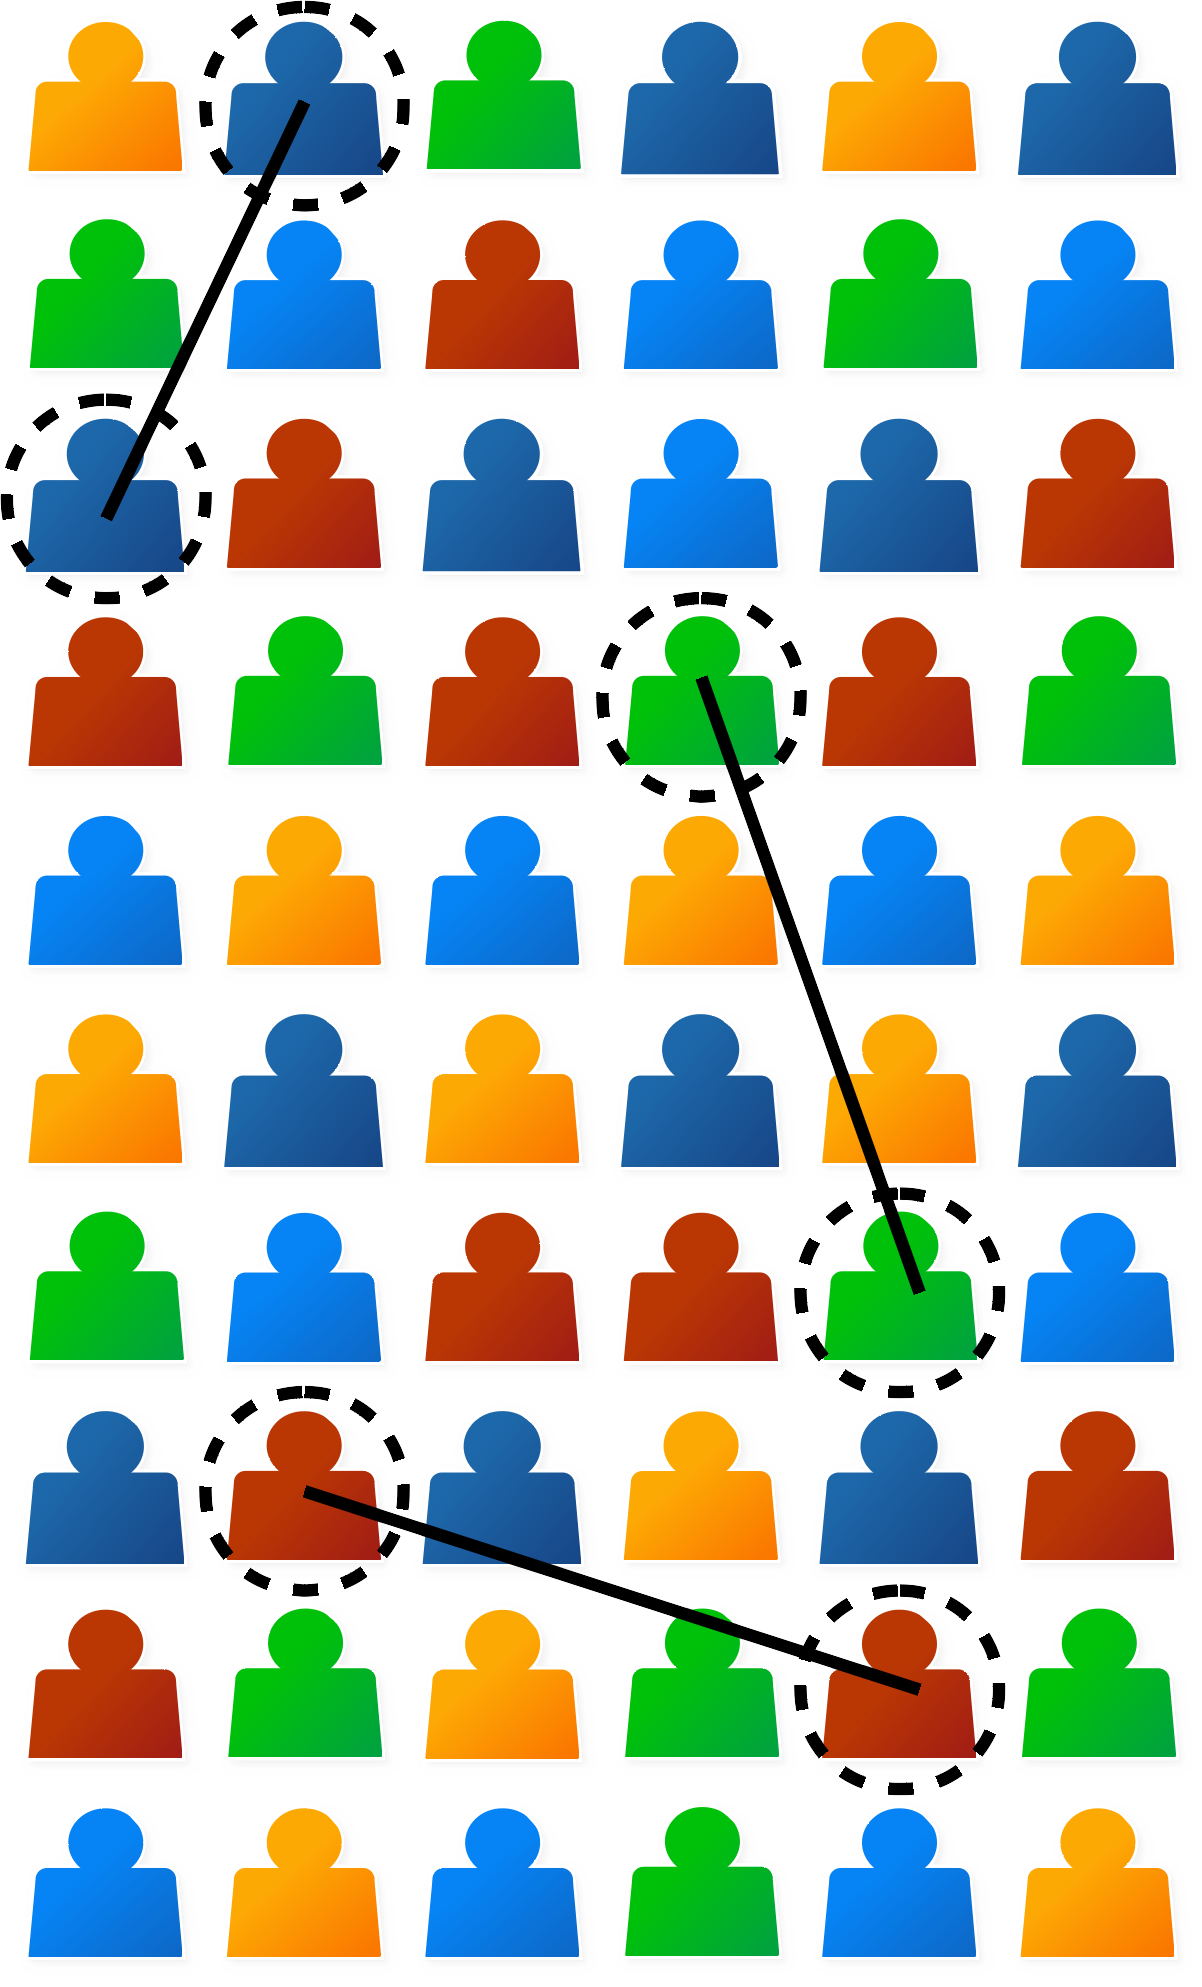
\includegraphics[width=\maxwidth{.35\linewidth}]{gfx/07-06}
	\caption{Matched Pair Sampling}
	\label{07:fig06}
\end{figure}

\textbf{Multi-stage Sampling} The sampling techniques described previously are all examples of single-stage sampling; however, they can be combined to conduct multi-stage sampling. For instance, a list of firms can be stratified based on size and then a systematic sampling can be conducted within each stratum. This would be a two-stage combination of stratified and systematic sampling. As a second example, a cluster of school districts in the state of Florida could be constructed and then a simple random sample of schools taken within each cluster, then a simple random sample of grade levels within each school, and, finally, a simple random sample of students taken from each grade level. This would constitute a four-stage sampling process consisting of cluster and simple random sampling.

\section{Sampling in Qualitative Research}

Qualitative researchers typically make sampling choices that enable them to deepen their understanding of the phenomenon being studied. \Gls{nonprobibilitysampling} sampling is a sampling technique in which some units of the population have zero chance of selection or where the probability of selection cannot be accurately determined. Typically, units are selected based on certain non-random criteria, such as quota or convenience. Because selection is not random, the sampling error cannot be estimated in non-probability sampling, and it may be subject to sampling bias. Also, the samples will not exhibit a normal distribution so statistics like mean and standard deviation are of no value. As a result, information from a non-probability sample cannot be generalized back to the entire population. 

Non-probability samples are ideal during the design phase of a research project. For example, a survey can be administered to only a few people who seem to resemble the population being investigated in order to help work out problems with the survey. A non-probability sample is also useful for some exploratory research project where the goal is to determine if there is a need to conduct a more extensive project. Researchers also use non-probability sampling as the primary means of data collection in extensive qualitative research projects where the researcher's goal is in-depth, \gls{idiographic} understanding rather than more general, \gls{nomothetic} understanding. Thus, researchers who are interested in contributing to the theoretical understanding of some phenomenon might use non-probability samples. 

Types of non-probability sampling techniques include the following.

\textbf{Convenience Sampling} This is sometimes called ``accidental'' or ``opportunity'' sampling and is a technique in which a sample is drawn from that part of the population that is close to hand, readily available, or convenient. For instance, if a researcher stood outside a shopping center and surveyed shoppers as they walk in it would form a convenience sample. This is a non-probability sample because shoppers at other shopping centers are systematically excluded from the survey. The results of the survey may reflect the unique characteristics of this particular shopping center, such as the nature of its stores, the demographic profile of its patrons, or its location, but would not be representative of the opinions of the shopper population at large. Hence, the scientific generalizability of such observations will be very limited. Other examples of convenience sampling are sampling students registered in a certain class or sampling patients arriving at a certain medical clinic. This type of sampling is most useful for pilot testing, where the goal is instrument testing or measurement validation rather than obtaining generalizable inferences.

Figure \ref{07:fig07} illustrates convenience sampling where the researcher in the top left corner only samples the nearby elements and ignores the rest.

\begin{figure}[H]
	\centering
	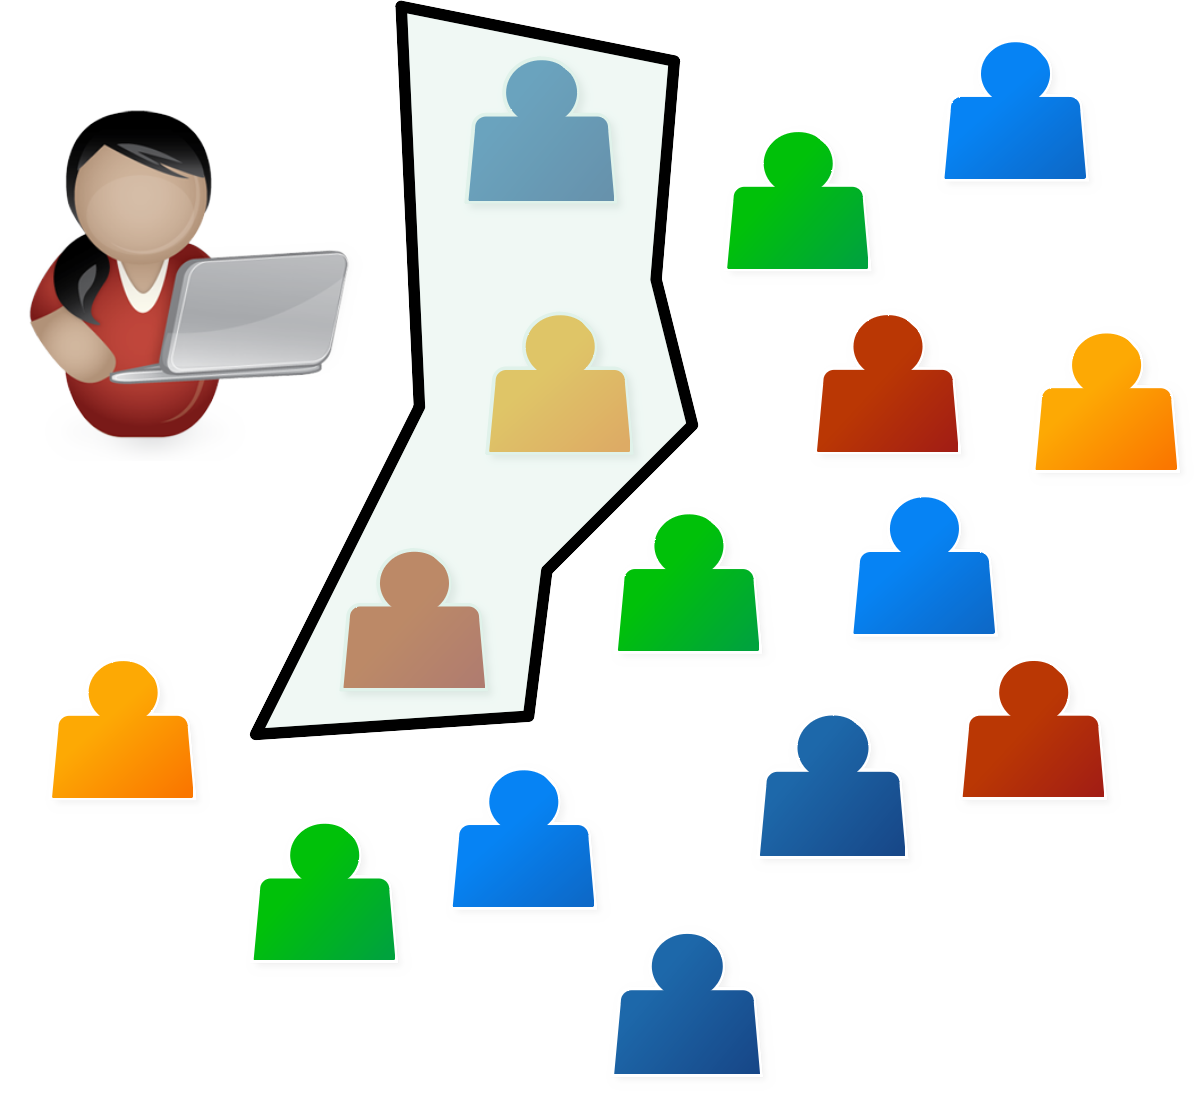
\includegraphics[width=\maxwidth{.35\linewidth}]{gfx/07-07}
	\caption{Convenience Sampling}
	\label{07:fig07}
\end{figure}

\textbf{Quota Sampling} In this technique, the population is segmented into mutually exclusive subgroups (just as in stratified sampling), and then a non-random set of observations is chosen from each subgroup to meet a predefined quota. In proportional quota sampling, the proportion of respondents in each subgroup should match that of the population. For instance, if the American population consists of 70\% Caucasians, 15\% Hispanic-Americans, and 13\% African-Americans, and researchers wished to understand their voting preferences in an sample of $ 100 $ people, they could stand outside a shopping center and ask people their voting preferences. But they would have to stop asking Hispanic people when they have $ 15 $ responses from that subgroup (or African-Americans when they have $ 13 $ responses) even as they continue sampling other ethnic groups. The goal is that the ethnic composition of the sample matches that of the general American population. Non-proportional quota sampling is less restrictive in that it does not have to achieve a proportional representation but does, perhaps, meet a minimum size in each subgroup. In this case, researchers may decide to have $ 50 $ respondents from each of the three ethnic subgroups (Caucasians, Hispanic-Americans, and African-Americans) and then stop when the quota for each subgroup is reached. Neither type of quota sampling will be representative of the American population, since depending on whether the study was conducted in a shopping center in New York or Kansas, the results may be entirely different. The non-proportional technique is even less representative of the population but may be useful in that it allows capturing the opinions of small and underrepresented groups through oversampling.

Figure \ref{07:fig08} illustrates quota sampling. In this case, a random sample is drawn from each of the subgroups but the larger subgroups have more samples than the smaller subgroups.

\begin{figure}[H]
	\centering
	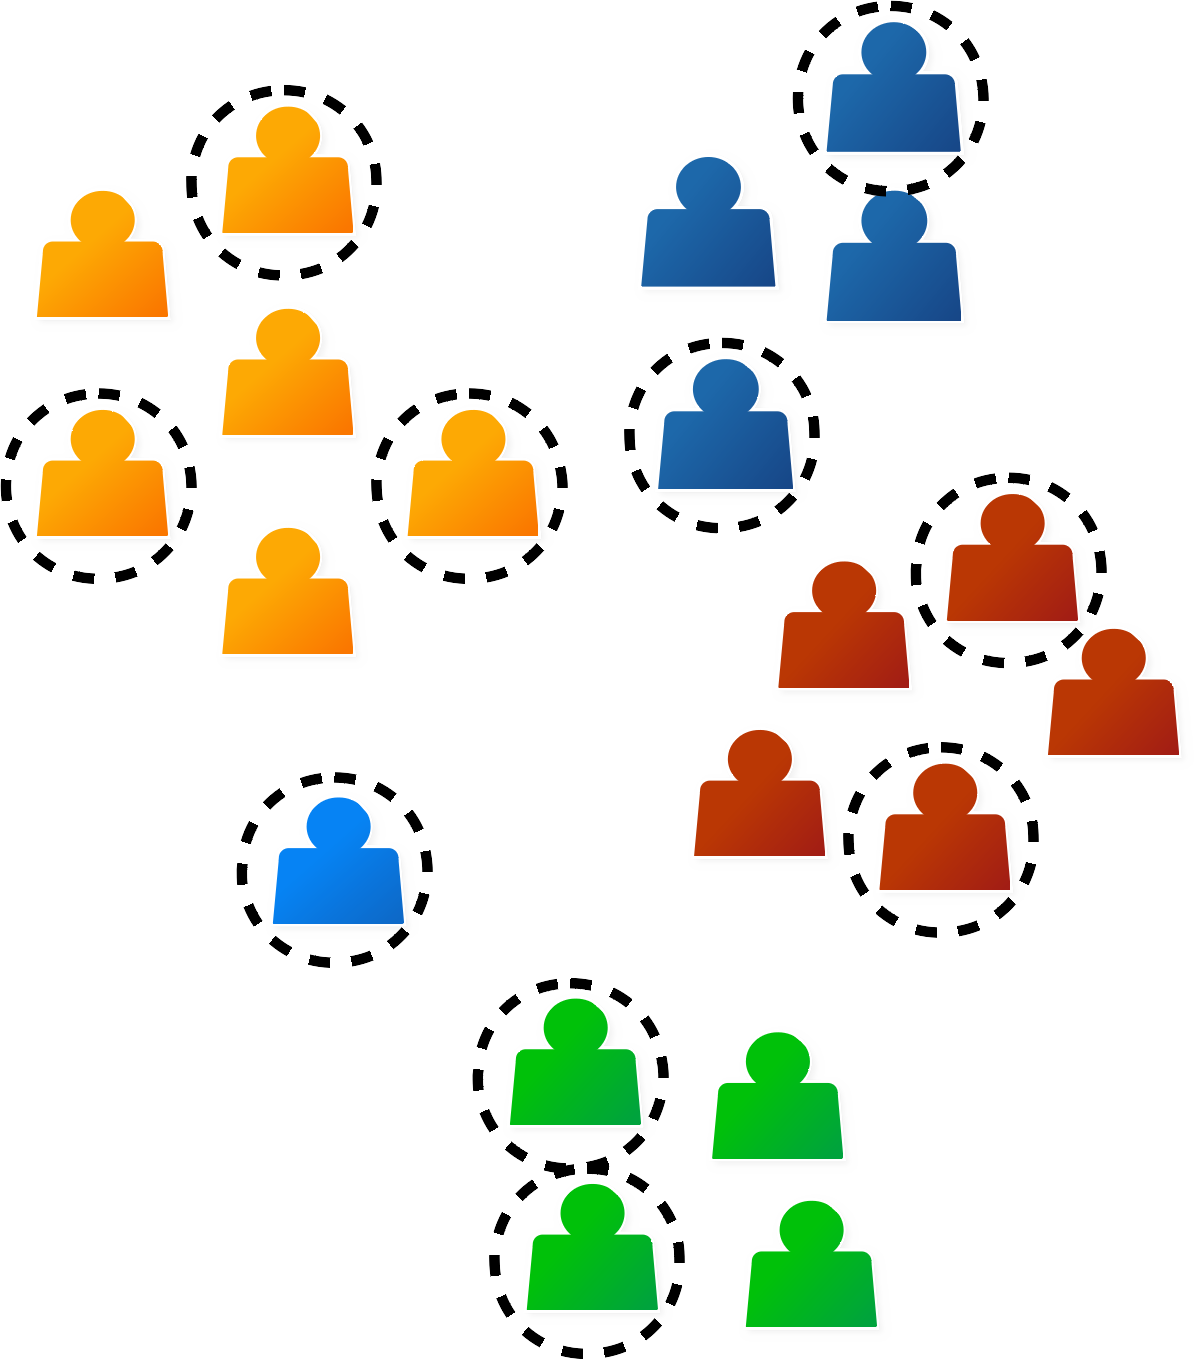
\includegraphics[width=\maxwidth{.35\linewidth}]{gfx/07-08}
	\caption{Quota Sampling}
	\label{07:fig08}
\end{figure}

\textbf{Snowball Sampling} In snowball sampling, a researcher starts by identifying a few respondents who match the criteria for inclusion in the study, and then asks those respondents to recommend others they know who would also meet the selection criteria. Snowball sampling is sometimes referred to as ``chain referral sampling'' since each respondent is also asked to provide the names of other potential respondents. After a few rounds, the researcher would have a large number of respondents, like a snowball getting larger as it rolls down a mountain. For example, if a researcher wishes to survey computer network administrators but only knows one or two then those people could recommend their peer network administrators and that group could recommend still others. Although this method hardly leads to representative samples, it may sometimes be the only way to reach hard-to-reach populations or when no sampling frame is available.

Figure \ref{07:fig09} illustrates snowball sampling. In this case, the researcher asked only one person, who recommended one other, who recommended two more, and so forth. In the end, the researcher sampled eight people but had only one to start the process.

\begin{figure}[H]
	\centering
	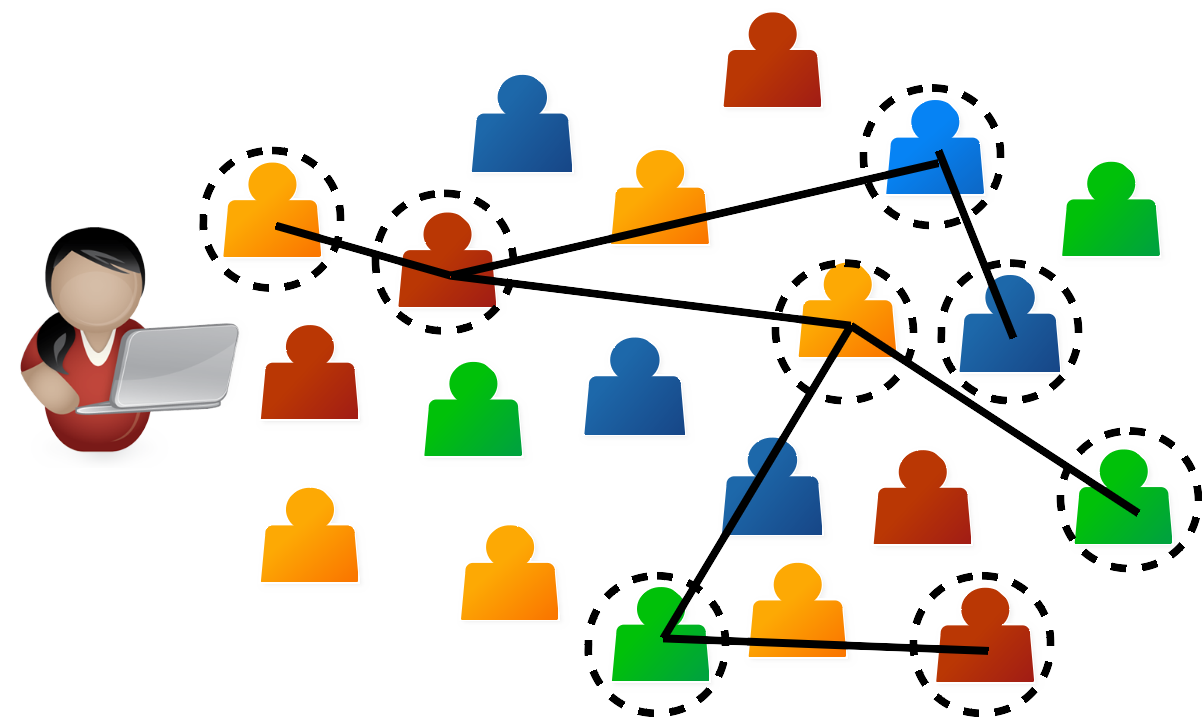
\includegraphics[width=\maxwidth{.35\linewidth}]{gfx/07-09}
	\caption{Snowball Sampling}
	\label{07:fig09}
\end{figure}

\textbf{Purposive Sampling} To draw a purposive sample, a researcher begins with specific perspectives to examine and then seeks research participants who exhibit the full range of perspectives. For example, a researcher studying students' satisfaction with their living quarters on campus would want to be sure to include students who stay in each of the different types or locations of on-campus housing. If only students from one of the ten dorms on campus are included then important details about the experiences of students who live in the other nine dorms would be missed. 

\textbf{Expert Sampling} This is a technique where respondents are chosen in a non-random manner based on their expertise on the phenomenon being studied. For instance, in order to understand the impacts of a new governmental policy such as the \textit{Sarbanes-Oxley Act}, a group of corporate accountants who are familiar with this act would be sampled. The advantage of this approach is that since experts tend to be more familiar with the subject matter than nonexperts, opinions from a sample of experts are more credible than a sample that includes both experts and non-experts, although the findings are still not generalizable to the overall population at large.


\section{Statistics of Sampling}

The preceding discussion introduced terms such as population, parameter, sample statistic, and sampling bias. This section defines these terms, and others, and illustrates how they are used and reported in a research project.

For this discussion, consider the data seen in Figure \ref{07:fig10}. This is a data set that represents the responses to a restaurant web survey such as is common in many fast food places. In this data, the attributes (columns) are a customer identification, the store number, the date and time a purchase was recorded, the purchase made (in coded form), and the answers to four questions, Q1-Q4. One column, illustrated in green, represents all responses to a single attribute, Q1 in this case. One observation (row) is highlighted in blue and represents all of the responses by a single customer.

\begin{figure}[H]
	\centering
%	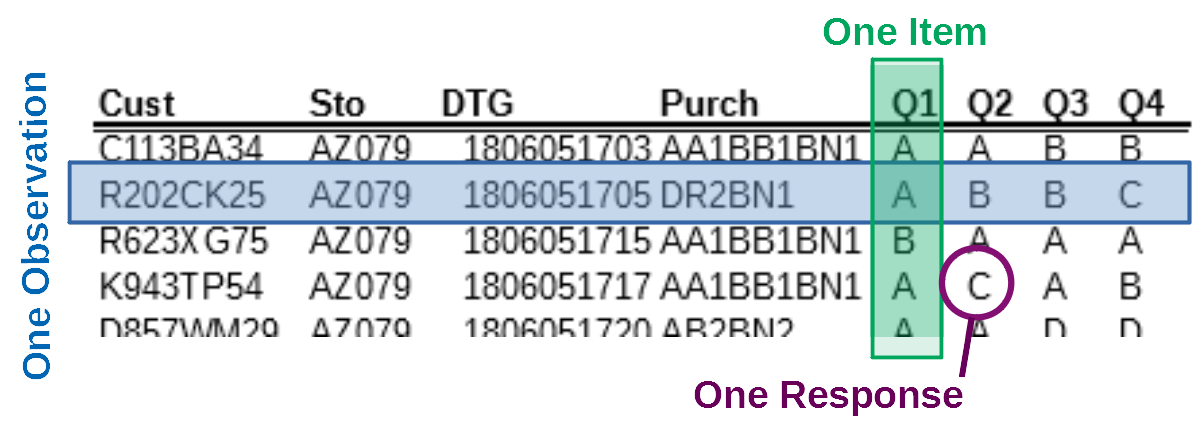
\includegraphics[width=\maxwidth{.95\linewidth}]{gfx/07-10}
	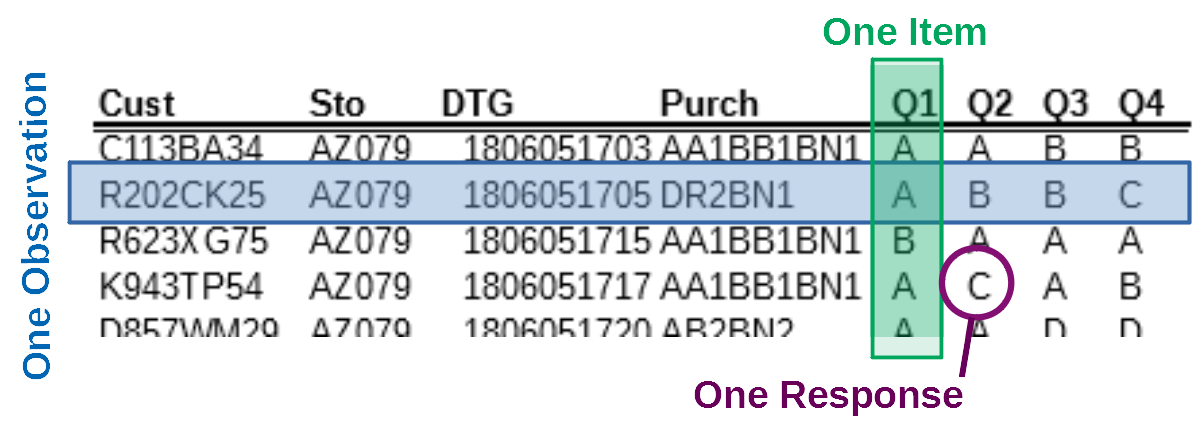
\includegraphics[]{gfx/07-10}
	\caption{Statistics Terms}
	\label{07:fig10}
\end{figure}

A specific observation of a phenomenon, such as a person's answer to a item Q2, is called a \textit{response}. In other words, a response is one point of measurement provided by a sampled unit (a customer). Researchers would expect each respondent to potentially provide different responses to the items in a survey. All responses for a single item, or a single column of data, can be analyzed in many different ways. If the item has \gls{nominaldata} data, that is, data that are in categories, then the responses can be graphed into a frequency distribution based on their frequency of occurrences. For the survey results in \ref{07:fig10}, the responses to Q2 can only be A, B, C, or D since those were the only selections possible; and that makes Q2 \gls{nominaldata} data. A frequency distribution for Q2 could look something like Figure \ref{07:fig12}.

\begin{figure}[H]
	\centering
	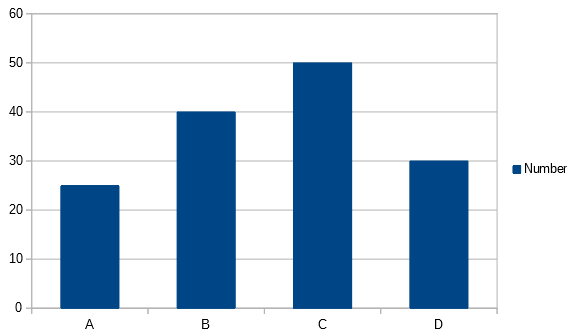
\includegraphics[width=\maxwidth{.95\linewidth}]{gfx/07-12}
	\caption{Frequency Chart}
	\label{07:fig12}
\end{figure}

Thus, the researcher could report that $ 40 $ people selected response B while $ 50 $ selected response C. If a sample has a large number of responses, the frequency distribution tends to resemble a normal distribution and that can then be used to estimate overall characteristics of the entire sample. \Gls{continuousdata}, such as measurements, can have various characteristics calculated, like the sample mean or standard deviation. These sample estimates are called sample statistics (a ``statistic'' is a value that is estimated from observed data). 

Populations also have means and standard deviations that could be obtained if we could sample the entire population; however, since the entire population can usually not be sampled, population characteristics are always unknown and are called population parameters (not ``statistic'' because they are not statistically estimated from data). Sample statistics may differ from population parameters if the sample is not perfectly representative of the population. For example, the sample mean may be $ 45 $ while the population parameter is $ 48 $, and the difference between the two is called ``sampling error.'' Theoretically, if sample size could be gradually increased so the sample size approaches that of the population then the sampling error will decrease and a sample statistic will increasingly approximate the corresponding population parameter. In reality, though, it is usually not possible to have a sample size equal to the population.

If a sample is truly representative of the population, then the estimated sample statistics should be identical to corresponding population parameters and to estimate how closely those align a sampling distribution is used. 

\begin{figure}[H]
	\centering
%	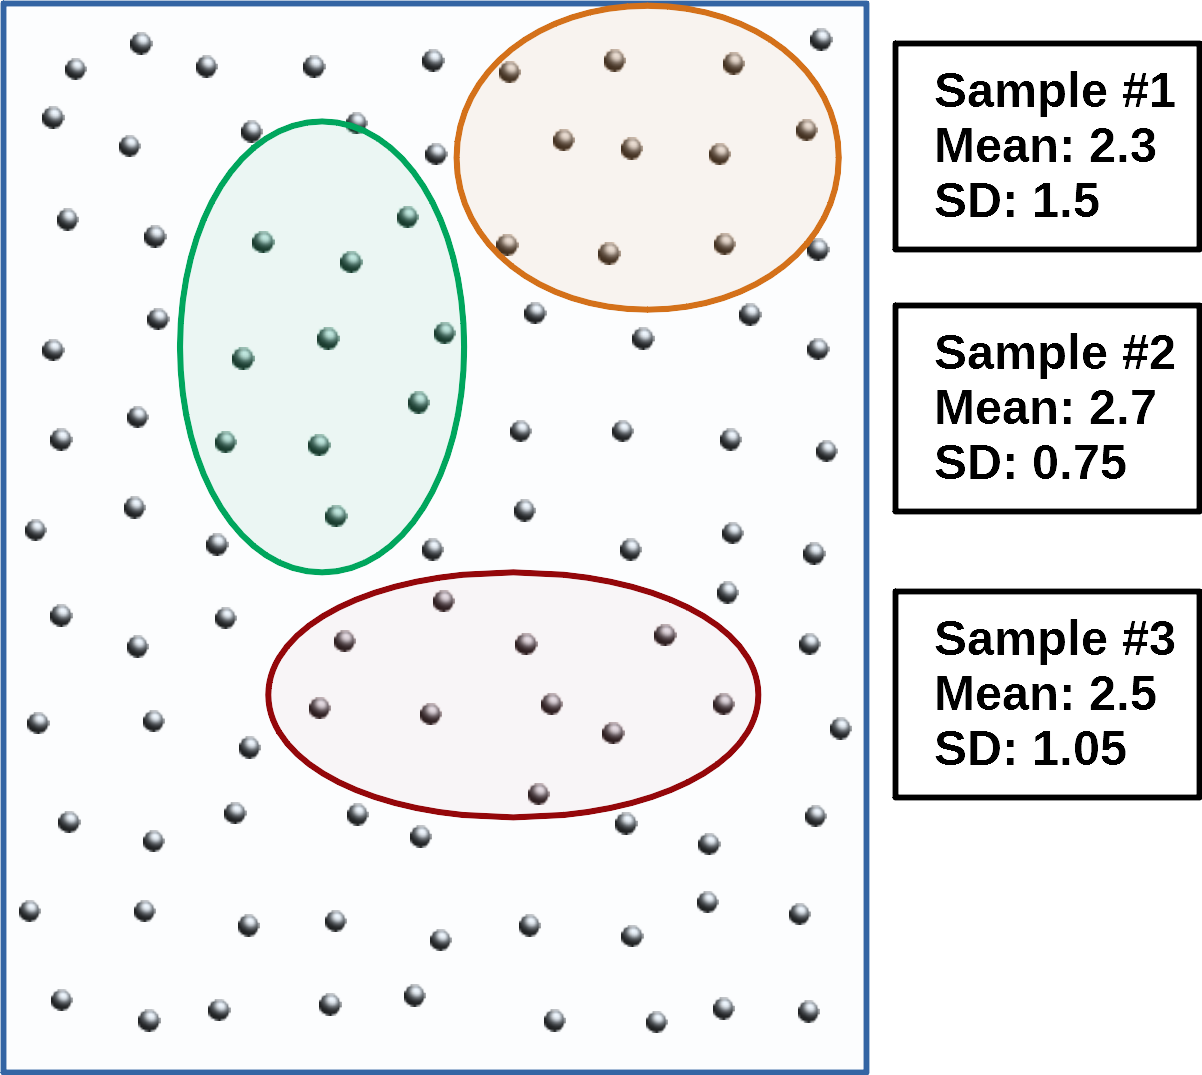
\includegraphics[width=\maxwidth{.95\linewidth}]{gfx/07-13}
	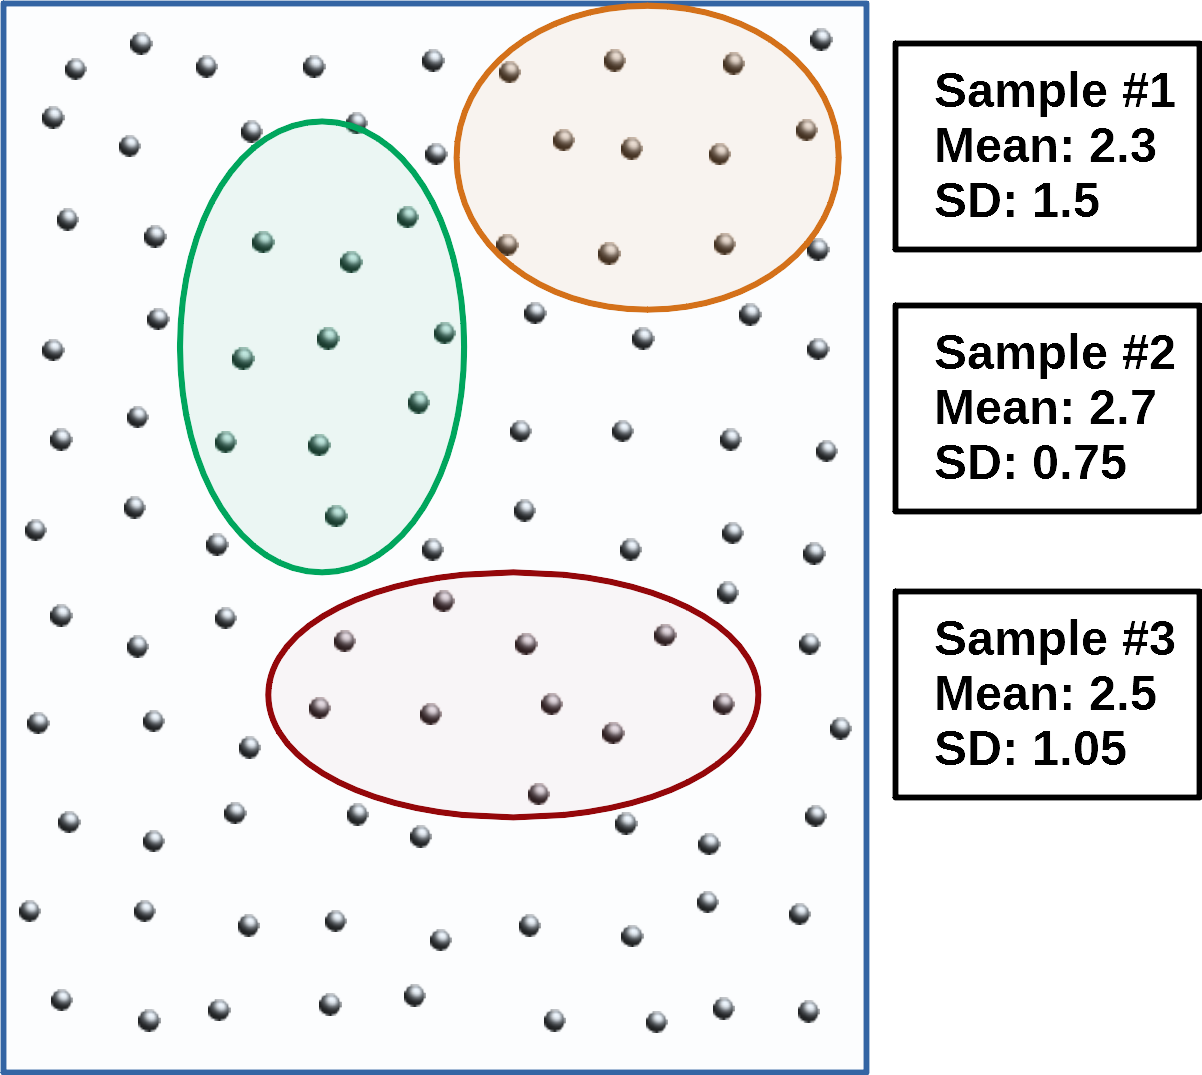
\includegraphics[]{gfx/07-13}
	\caption{Sample Statistics}
	\label{07:fig13}
\end{figure}

Figure \ref{07:fig13} illustrates the data from a research project. Imagine that three different random samples are drawn from the population and the mean and standard deviation are calculated for each sample. If each random sample was perfectly representative of the population, then the means and standard deviations from the three samples will be identical and equal to the population parameter. But this is extremely unlikely since each random sample will likely constitute a different subset of the population so their calculated statistics will be slightly different from each other. 

If the mean of the three sample means is calculated then it would be possible to also calculate the variability (or spread) of those means and that calculation is called the \textit{standard error of the mean}. The method to calculate that number is beyond the scope of this book, but the standard error of the mean for Figure \ref{07:fig13} is 0.115.\footnote{Students interested in how this number was derived can find help online. One source is an online calculator: \url{https://www.calculator.net/standard-deviation-calculator.html} and a good non-technical explanation can be found at \url{http://www.assess.com/standard-error-mean/}  } 

As the number of samples drawn from the population increases the variance between the means of those samples tends to decrease and they approach the mean of the entire population. Also, as the number of samples increases the standard error of the mean decreases and approaches zero. The mean value of a sample is presumed to be an estimate of the population parameter and the standard error of the mean makes it is possible to estimate \textit{confidence intervals} for how well the statistical mean predicts the population parameter. Since the standard error is similar to the standard deviation for a group of samples, it can be said that:

\begin{itemize}
	\item (Sample statistic + one standard error) represents a $ 68\% $ confidence interval for the population parameter.
	\item (Sample statistic + two standard errors) represents a $ 95\% $ confidence interval for the population parameter.
	\item (Sample statistic + three standard errors) represents a $ 99\% $ confidence interval for the population parameter.
\end{itemize}

In Figure \ref{07:fig13}, the mean of the three samples is $ 2.5 $ and the standard error is $ 0.115 $. Therefore, any sample mean in the range of $ 2.385-2.615 $ has a $ 68\% $ chance of predicting the population mean, any sample mean in the range of $ 2.27-2.73 $ has a $ 95\% $ chance of predicting the population mean, and any sample mean in the range of $ 2.155-2.845 $ has a $ 99\% $ chance of predicting the population mean. Since sample one falls in the $ 95\% $ confidence band a researcher could predict that $ 2.3 $ (the mean of that sample) predicts the mean of the entire population with a $ 95\% $ confidence level.

\section{Sample Size}

When working with sampling, one of the first questions researchers face is the sample size. In other words, how many observations are needed to have a useful sample. In general, the larger the sample the more accurately it will represent the population and the more robust the statistical analysis is possible. Unfortunately, the answer to the question about sample size is a bit nebulous. One rule of thumb that many researchers mention is a minimum of $ 30 $, but that is a gross oversimplification and does not work well except in classroom-size projects for university students. When determining an appropriate sample size, a number that is too small may exclude parts of the population while a number that is too large may become unwieldy for the researcher. 

Determining an appropriate sample size is a mix of both mathematics and experience. There are formulas that will help researchers determine a good sample size, but those must be tempered with experience and an understanding of the population being studied. For example, if a formula indicated that a sample size of $ 250 $ is appropriate for a population of $ 500 $ people but the researcher happens to know that the population is very diverse with many racial or ethnic groups then the sample may need to be increased to ensure that all groups are fairly represented.

To make researcher's jobs easier, numerous sample size tables have been published and it is easy to refer to these tables to determine a good sample size. Figure \ref{07:fig14} shows a very simple such table\cite{israel1992determining}.

\begin{figure}[H]
	\centering
	%	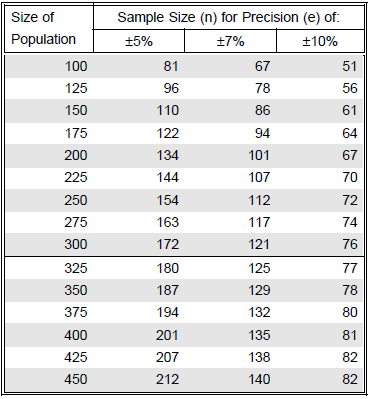
\includegraphics[width=\maxwidth{.35\linewidth}]{gfx/07-14}
	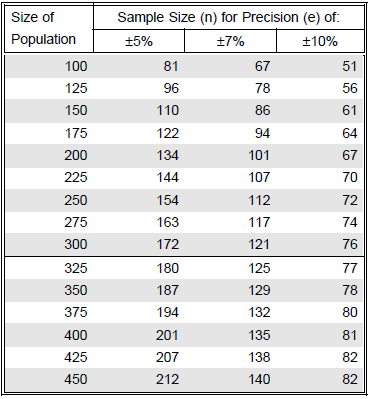
\includegraphics[width=4in]{gfx/07-14}
	\caption{Sample Size For Confidence Level of 95\%}
	\label{07:fig14}
\end{figure}

In the table in Figure \ref{07:fig14}, the confidence level is $ 95\% $ for all values. This is a typical confidence level and is commonly used in the statistical analysis of a data set. Very frequently, that confidence level is expressed as a \gls{pvalue} of $ 0.05 $. Precision, in this case, is defined as how close the estimates from different samples are to each other. The smaller the precision then the closer the values in each sample will be to each other and, presumably, to the population parameter. As an example from the table in Figure \ref{07:fig14}, if a researcher were conducting a survey for a population of $ 400 $ and desired $ 5\% $ precision then $ 201 $ samples would need to be taken.

\section{A Word of Caution}

It is easy to overlook the need to ask important questions about where research participants come from and how they are identified for inclusion in a research project, in other words, how the sample was determined. It is easy to focus only on the interesting ``stuff'' in the findings, but understanding the procedures used for selecting study participants is critical.

Students who have ever taken an introductory psychology or sociology class at a large university are very frequently drafted into research projects since that is an easy group for graduate students to access. But that access comes at a cost: sample representativeness. One study of top academic journals in psychology found that over two-thirds ($ 68\% $) of participants in studies published by those journals were based on samples drawn in the United States\cite{arnett2008neglected} Further, the study found that two-thirds of the work that derived from United States samples published in the Journal of Personality and Social Psychology was based on samples made up entirely of American undergraduates taking psychology courses.

These findings raise an interesting the question: What do we actually learn from social scientific studies and about whom do we learn it? That is exactly the concern raised by Joseph Henrich and colleagues\cite{henrich2010most} who point out that behavioral scientists very commonly make sweeping claims about human nature based on samples drawn only from \textit{WEIRD} (Western, Educated, Industrialized, Rich, and Democratic) societies, and often based on even narrower samples, as is the case with many studies relying on samples drawn from college classrooms. As it turns out, many robust findings about the nature of human behavior when it comes to fairness, cooperation, visual perception, trust, and other behaviors are based on studies that excluded participants from outside the United States and sometimes excluded anyone outside the college classroom. This certainly raises questions about what we really know about human behavior as opposed to that of United States undergraduate behavior. Of course not all research findings are based on samples of \textit{WEIRD} folks like college students. But even then it is important to pay attention to the samples on which studies are based and the claims that are being made about to whom those studies apply.

In the preceding discussion, the concern is with researchers making claims about populations other than those from which their samples were drawn. A related, but slightly different, potential concern is sampling bias. Bias in sampling occurs when the elements selected for inclusion in a study do not represent the larger population from which they were drawn. For example, an on-line poll conducted by a newspaper asking for an opinion about some local issue will certainly not represent the public since those without access to computers or the Internet, those who do not read that paper's website, and those who do not have the time or interest will not answer the question.

Another thing to keep in mind is that just because a sample may be representative in all respects that a researcher thinks are relevant, there may be aspects that are relevant that did not occur to the researcher. For example, peoples' phones would seem to have little to do with their voting preferences but had pollsters making predictions about the results of the $ 2008 $ presidential election not been careful to include both cell phone and land line households in their surveys, it is possible that their predictions would have underestimated Barack Obama's lead over John McCain because Obama was much more popular among cell-only users than McCain\cite{keeter2008calling}.

When evaluating a research report, remember that sample quality is determined only by the sample actually obtained, not by the sampling method itself. A researcher may set out to administer a survey to a representative sample by correctly employing a random selection technique, but if only a handful of the people sampled actually respond to the survey, the researcher will have to be very careful about the claims made. Another thing to keep in mind is that researchers discuss the implications of their findings as though they apply to some group other than the population actually sampled. This tendency is usually innocent since it is human nature to inflate the applicability of the findings; but consumers of those findings must be attentive to this sort of (hopefully unintentional) bait and switch. 

At their core, questions about sample quality should address who has been sampled, how they were sampled, and for what purpose they were sampled. Being able to answer those questions will improve understanding of the research results.

\section{Summary}

\begin{itemize}
	\setlength{\itemsep}{0pt}
	\setlength{\parskip}{0pt}
	\setlength{\parsep}{0pt}
	
	\item To be provided.
	\item To be provided.
	
\end{itemize}
